\documentclass{article}
\usepackage{graphicx} 
\usepackage{cite}
\usepackage{amsmath,amssymb,amsfonts}
\usepackage{algorithmic}
\usepackage{textcomp}
\usepackage{xcolor}
\usepackage{booktabs}
\usepackage{arydshln}
\usepackage[a4paper, margin=1in]{geometry}
\usepackage{algorithm}
\usepackage{algorithmic}
\usepackage{placeins}
\usepackage{float}
\usepackage{subcaption}

\title{Laboratory 5: Rigid and Non-Rigid Structure from Motion}
\author{Víctor Brull Rico \and Guillem Martínez Sambola}
\date{June 1, 2026}

\begin{document}

\maketitle

\section{Introduction}

Structure from Motion (SfM) is a key area of study in computer vision. It focuses on recovering both the 3D structure of an object or scene and the motion parameters of a camera from a sequence of 2D image points. Standard rigid SfM assumes that the physical coordinates of the target points do not change relative to each other over time. However, many real-world tasks involve dynamic shapes, such as human bodies, moving garments, or facial expressions. This requires Non-Rigid Structure from Motion (NRSfM) formulations.

This report presents our work for Laboratory 5, which covers three core implementations: rigid factorization using orthographic cameras, non-rigid shape optimization under low-rank shape models, and non-rigid trajectory-space factorization using a predefined Discrete Cosine Transform (DCT) basis. We analyze how parameters like the rank $K$ and geometric smooth priors influence 3D tracking and reconstruction accuracy. Finally, we review recent deep learning-based approaches that replace linear subspace matrices with continuous implicit coordinates.

\section{Methods}
\label{sec:Methods}

\subsection{2D Tracking Data and Measurement Matrix}

The script \texttt{visualize\_2Dtracking.m} loads the \emph{Dinosaur} monocular video sequence together with its per-frame 2D point annotations, plays the frames sequentially, and overlays the tracked landmarks as coloured markers. This visualization allows us to inspect tracking coverage, identify frames with missing observations, and develop intuition about the apparent 2D motion before constructing the measurement matrix.

From these annotations we build the measurement matrix $W \in \mathbb{R}^{2F \times P}$, where $F$ is the total number of frames and $P$ is the number of tracked points. Each consecutive pair of rows $(2f-1,\,2f)$ stores the horizontal ($u$) and vertical ($v$) pixel coordinates of all $P$ points in frame $f$:
\[
    W = \begin{pmatrix}
        u_{1,1} & \cdots & u_{1,P} \\
        v_{1,1} & \cdots & v_{1,P} \\
        \vdots  &        & \vdots  \\
        u_{F,1} & \cdots & u_{F,P} \\
        v_{F,1} & \cdots & v_{F,P}
    \end{pmatrix}.
\]
A binary visibility mask $D \in \{0,1\}^{F \times P}$ records which entries are actually observed; missing entries are excluded from all residual computations throughout the pipeline.

\begin{figure}[H]
\centering
\begin{subfigure}[b]{0.45\linewidth}
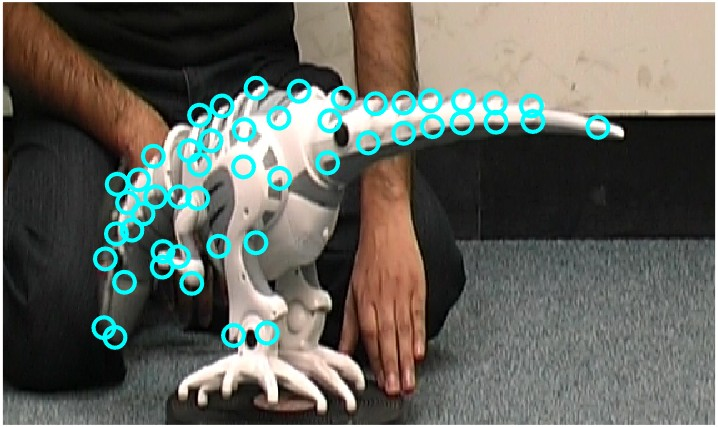
\includegraphics[width=\linewidth]{Figures/dinosaur_2Dtracking.jpg}
\end{subfigure}
\hfill
\caption{2D tracked points overlaid on a representative frame from the Dinosaur sequence.}
\label{fig:dinosaur_2Dtracking}
\end{figure}

\subsection{Rigid Structure from Motion by Factorization}

Under an orthographic camera model, after subtracting the per-frame centroid from $W$ to remove translation, the mean-free measurement matrix factorizes exactly as:
\[
    \tilde{W} = R\,S,
\]
where $R \in \mathbb{R}^{2F \times 3}$ stacks the two camera projection rows for every frame and $S \in \mathbb{R}^{3 \times P}$ is the (time-invariant) 3D shape matrix. Because $\tilde{W}$ has rank at most 3 under the rigidity assumption, a truncated SVD provides an initial factorization that is then corrected by a metric upgrade.

The function \texttt{rigidfactorization\_ortho.m} implements the following four steps:
\begin{enumerate}
    \item \textbf{Mean subtraction.} The per-frame centroid of the visible observations is computed and subtracted from each row pair of $W$, yielding the centred matrix $\tilde{W}$.
    \item \textbf{Rank-3 SVD.} The decomposition $\tilde{W} \approx U_3\,\Sigma_3\,V_3^T$ is computed retaining only the three largest singular values. Initial factors are set as $\hat{R} = U_3\,\Sigma_3^{1/2}$ and $\hat{S} = \Sigma_3^{1/2}\,V_3^T$.
    \item \textbf{Metric upgrade.} Orthonormality of the camera rows imposes quadratic constraints on a $3 \times 3$ symmetric upgrade matrix $G$ such that the corrected motion is $R = \hat{R}\,G^{-1/2}$. These constraints are linearized and solved by least squares; $G$ is then recovered via Cholesky decomposition.
    \item \textbf{Shape and rotation recovery.} The corrected rotation $R$ and shape $S = G^{1/2}\hat{S}$ are extracted, and per-frame rotation sub-matrices $R_f \in \mathbb{R}^{2 \times 3}$ are normalized to enforce exact orthonormality.
\end{enumerate}

The quality of the reconstruction is measured by the normalized 3D reconstruction error:
\[
    \epsilon_{3D} = \frac{\|\hat{S} - S_{\mathrm{gt}}\|_F}{\|S_{\mathrm{gt}}\|_F},
\]
where $S_{\mathrm{gt}}$ denotes the ground-truth shape after Procrustes alignment to the estimate. On the synthetic ogre sequence the method achieves $\epsilon_{3D} = 0.002865\%$, confirming that rigid factorization recovers the shape with negligible error when the rigidity assumption is satisfied.

\begin{figure}[H]
\centering
\begin{subfigure}[b]{0.35\linewidth}
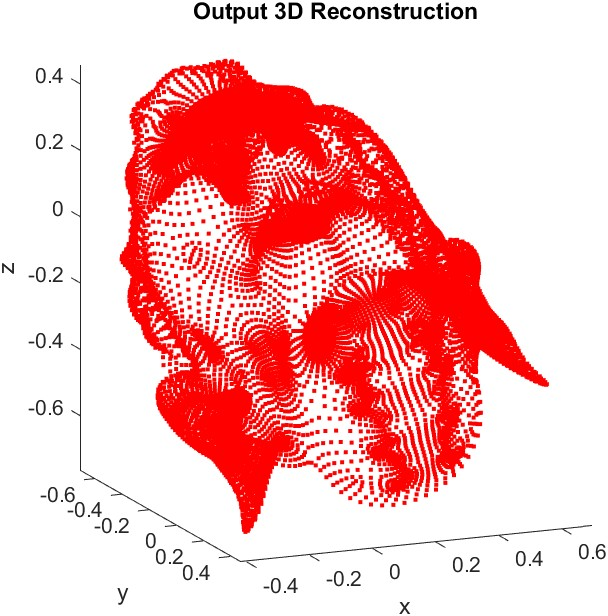
\includegraphics[width=\linewidth]{Figures/ogre3D_1.jpg}
\caption{Estimated 3D reconstruction}
\end{subfigure}
\hfill
\begin{subfigure}[b]{0.45\linewidth}
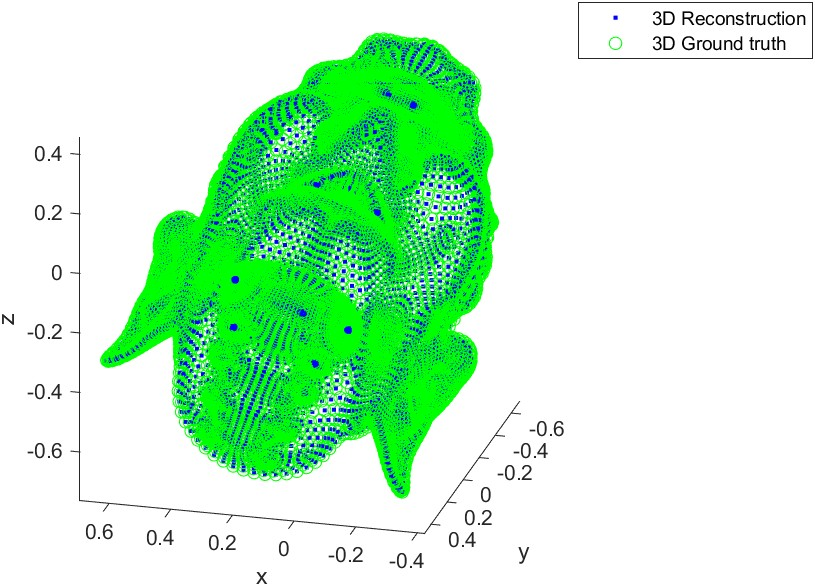
\includegraphics[width=\linewidth]{Figures/ogre3Dground.jpg}
\caption{Ground truth}
\end{subfigure}
\caption{3D reconstruction of the Ogre sequence using rigid orthographic factorization. Both views are obtained by rotating the point cloud with the \texttt{rotate3D} option.}
\label{fig:ogre_3Dreconstruction}
\end{figure}

\subsection{Non-Rigid Shape Space Optimization}

The non-rigid optimization implemented in this lab jointly estimates a compact time-varying 3D shape model and camera motion by minimizing a reprojection error together with optional temporal smoothness priors. The observed data is the measurement matrix $W\in\mathbb{R}^{2F\times P}$ (two image coordinates per frame, $F$ frames, $P$ tracked points). Under the orthographic approximation the forward model for point $p$ in frame $f$ is written as
\[
	\mathbf{w}_{f,p} = \mathbf{R}_f\,\mathbf{s}_{f,p} + \mathbf{t}_f,
\]
where $\mathbf{w}_{f,p}\in\mathbb{R}^2$ is the image observation, $\mathbf{R}_f\in\mathbb{R}^{2\times3}$ contains the camera rows, $\mathbf{t}_f\in\mathbb{R}^2$ is the translation, and $\mathbf{s}_{f,p}\in\mathbb{R}^3$ is the 3D location of point $p$ at frame $f$.

To model non-rigidity we parameterize each instantaneous shape as a linear combination of $K$ basis shapes:
\[
	\mathbf{s}_{f,p} = \sum_{k=1}^K L_{k,f}\,\mathbf{x}_{k,p},
\]
where $\mathbf{x}_{k,p}\in\mathbb{R}^3$ is the coordinates of point $p$ in basis $k$ and $L_{k,f}$ is the scalar coefficient active at frame $f$. Stacking the $K$ bases into $X\in\mathbb{R}^{3P\times K}$ and the frame coefficients into $L\in\mathbb{R}^{K\times F}$ yields the compact relation used by the code:
\[
	W_{2f-1:2f,:} = R_f\,\mathrm{reshape}(X\,L_{:,f},3,P) + t_f\mathbf{1}_P^T.
\]

\textbf{Parameter vector and conversion helpers.} The solver operates on one long parameter vector that follows the exact packing implemented by \texttt{model2vector.m} and undone by \texttt{vector2model.m}. The per-frame block has size $K+6$ and contains, in order, the $K$ coefficients $L_{:,f}$, a 4-component quaternion parameterizing rotation, and the two translations. The $F$ frame blocks are concatenated and the basis shapes are appended afterwards as $K$ blocks of size $3P$ each. This ordering makes the frame-local parameters contiguous and groups all basis coordinates by basis index.

\textbf{Cost function and residual ordering.} The data residual in \texttt{cost\_RXT.m} is computed by building the predicted 2D points $W_{\mathrm{pred}}$ and forming
\[
	e_{\mathrm{data}} = \mathrm{vec}(W_{\mathrm{pred}})^{}_{\mathcal{V}} - x,
\]
where $x$ is the vector of observed coordinates assembled in \texttt{nrsfm.m} via \texttt{A = W'}, \texttt{D = D'} and \texttt{projections = A(D(:)==1)}. Because both \texttt{A} and \texttt{D} are laid out as $P\times 2F$ matrices and then vectorized column-wise, the data residuals are ordered by coordinate ($u$ then $v$ for frame 1, $u$ then $v$ for frame 2, \ldots) and, inside each coordinate, by point index. This precise ordering is important because the Jacobian pattern must match it exactly.

\textbf{Temporal priors.} Two optional smoothness priors are appended to the residual vector and weighted in the cost:
\begin{itemize}
	\item \emph{Deformation smoothness} (coefficient prior): for each consecutive pair of frames a residual $e_{L,f}=L_{:,f}-L_{:,f+1}$ is added and scaled by \texttt{priors.coeff\_weight}. This penalizes rapid changes in the low-dimensional deformation coefficients.
	\item \emph{Motion smoothness} (camera prior): for each consecutive pair of frames a residual based on the change of the camera rows is added, implemented as $e_{R,f}=\|R_f-R_{f+1}\|_F / \|R_f\|_F$ and scaled by \texttt{priors.camera\_weight}. This penalizes abrupt camera rotations.
\end{itemize}

\textbf{Optimization details.} The problem is solved with Levenberg--Marquardt using \texttt{lsqnonlin}. To exploit sparsity and avoid computing unnecessary finite-difference columns, the solver receives a sparse Jacobian pattern through \texttt{opt.JacobPattern = JacobianPattern(...)}. Initialization is performed with a rigid factorization (\texttt{rigidfactorization\_ortho}); translations are initialized to the per-coordinate mean of $W$, the basis $X$ is seeded by copying the rigid shape into the $K$ basis blocks, and $L$ is initialized randomly. After convergence the vector is mapped back to structured $R$, $T$, $X$, $L$ to compute reprojection and 3D reconstruction results.

\textbf{Practical notes.} Derivatives with respect to coefficients $L_{k,f}$ and basis coordinates $X_{k,p}$ are straightforward (the predicted 2D measurement is linear in those variables once $R_f$ is fixed). Derivatives with respect to rotation parameters are handled implicitly by including the quaternion entries in the pattern. Translations act only on the corresponding coordinate (horizontal $u$ depends on $t_x$, vertical $v$ on $t_y$), which is reflected directly in the sparsity pattern.

\subsection{Creating the Jacobian Pattern}

The Jacobian pattern describes which unknown parameters influence each scalar residual. \texttt{JacobianPattern.m} builds that sparse pattern following exactly the residual and parameter packing described above. The key aspects are:

\begin{enumerate}
	\item \textbf{Pattern size calculation.} The number of data rows equals twice the number of visible (measured) points, so the code preallocates
		\[ \#\text{rows} = 2\,\mathrm{nnz}(vij) + (\text{coeff\_prior} + \text{camera\_prior})\,(F-1), \]
		where the latter term accounts for the possible $F-1$ prior residuals for each enabled prior. The number of columns is exactly the parameter vector length
		\[ \#\text{cols} = (K+6)F + K\,(3P). \]

	\item \textbf{Column indexing} (explicit formulas used in the code):
		\begin{itemize}
			\item Per-frame block size $B = K+6$.
			\item Coefficient column for $L_{k,f}$: $c_{L_{k,f}} = (f-1)B + k$.
			\item Quaternion component $i$ of frame $f$: $c_{q_{i,f}} = (f-1)B + K + i,\; i=1\ldots4$.
			\item Translation columns of frame $f$: $c_{t_{x,f}} = (f-1)B + K + 5$ and $c_{t_{y,f}} = (f-1)B + K + 6$.
			\item Basis block start: $X_{\mathrm{base}} = (K+6)F$.
			\item Basis $k$, point $p$, coordinate $j\in\{1,2,3\}$: $c_{X_{k,p,j}} = X_{\mathrm{base}} + (k-1)3P + 3(p-1) + j$.
		\end{itemize}

	\item \textbf{Row construction (data term).} The implementation loops over coordinate index $c=1\ldots 2F$ (odd $c$ $\Rightarrow$ horizontal coordinate $u$ of frame $f=(c+1)/2$, even $c$ $\Rightarrow$ vertical $v$ of frame $f=c/2$) and then over points $p=1\ldots P$. If the point is visible (\texttt{vij(f,p)}), the current residual row is created and the code marks as non-zero the columns
		\[ [L_{:,f},\; q_{:,f},\; t_{\text{relevant}},\; X_{\text{all bases for point }p}] \]
		by setting \texttt{J(row,cols)=1}. This mirrors the analytic dependency: the measurement depends on the $K$ coefficients at that frame, the frame rotation, the matching translation component, and the $3K$ coordinates of point $p$ across all bases.

	\item \textbf{Row construction (priors).} Once all data rows are created, the code appends deformation prior rows (if enabled) where each prior row depends only on the coefficient columns of frames $f$ and $f+1$, and then appends camera prior rows where each depends only on the quaternion columns of frames $f$ and $f+1$. This ordering matches the residual stacking in \texttt{cost\_RXT.m} and guarantees pattern alignment.
\end{enumerate}

This explicit and consistent mapping between parameter packing (\texttt{model2vector.m}) and residual construction (\texttt{nrsfm.m} / \texttt{cost\_RXT.m}) is what makes the pattern exact: it marks every column that can give a non-zero partial derivative for a given residual and leaves the rest zero. The solver therefore computes only the required finite-difference Jacobian columns, which both speeds up the optimization and reduces memory usage. For quick verification the function also draws the pattern with \texttt{spy(J,3)}, letting the user visually confirm that data rows connect to the expected per-frame blocks and that prior rows only cross the intended coefficient or quaternion blocks.

\subsection{Non-Rigid Trajectory Factorization Framework}

Instead of representing non-rigid structures via linear combinations of shape bases, the trajectory-space framework models the temporal path of each point using a predefined Discrete Cosine Transform (DCT) basis matrix $C \in \mathbb{R}^{F \times K}$. This enforces low-frequency temporal smoothness on the coordinates directly.

\subsubsection{Implementation Details and Algorithmic Flow}

The complete script execution flow for solving and visualizing the trajectory factorization is implemented through the following computational steps:
\begin{enumerate}
    \item \textbf{Initial Subspace Decomposition:} The measurement matrix $W$ is centralized and factored via an initial Singular Value Decomposition truncated to a rank of $3K$. This outputs an initial uncalibrated camera motion matrix $\hat{R}_{sh} \in \mathbb{R}^{2F \times 3K}$ and an uncalibrated trajectory coefficient state matrix $\hat{X} \in \mathbb{R}^{3K \times P}$.
    \item \textbf{Metric Calibration:} A metric upgrade step solves for a regularized transformation matrix $Q \in \mathbb{R}^{3K \times 3K}$ by imposing orthographic camera constraints. The true metric camera rotation parameters $R \in \mathbb{R}^{2F \times 3}$ are subsequently isolated and recovered frame-by-frame via the auxiliary script \texttt{recoverR.m}.
    \item \textbf{Closed-Form Regression Fitting:} With the camera parameters $R$ known, the spatial basis tensor $G \in \mathbb{R}^{2F \times 3K}$ is formed by computing the Kronecker product or broadcasted element-wise multiplication between camera views and the temporal DCT matrix rows ($G = R \cdot C$). The final dense tracking trajectory coefficients matrix $D \in \mathbb{R}^{3K \times P}$ is resolved globally using ordinary linear least squares:
    \begin{equation}
    D = (G^T G)^{-1}G^T W
    \end{equation}
    The time-varying 3D shape matrix configuration is finally reconstructed via $X = C \cdot D$.
    \item \textbf{Frame-by-Frame Proportional Re-projection:} To overlay the tracking solution visually onto the original video image files in \texttt{visualize\_2Dtracking.m}, bulk matrix dimensions are broken down inside an active processing loop over $F$ frames. At each index step $i$, a localized $2 \times P$ coordinate map is evaluated safely without dimension conflict:
    \begin{equation}
    W_{frame\_est} = R_{frame} \cdot S_{frame} + T_{frame} \cdot \mathbf{1}_{1 \times P}
    \end{equation}
    where $R_{frame} = R(2i-1:2i, :)$, $S_{frame} = X(3i-2:3i, :)$, and $T_{frame} = T(2i-1:2i, :)$.
\end{enumerate}

\subsection{Learning-Based Non-Rigid Structure from Motion}

Finally, we review the learning-based framework proposed in \textit{Neural Dense Non-Rigid Structure from Motion with latent space constraints} \cite{sidhu2020neural}. This approach bypasses traditional linear subspace models by utilizing an unsupervised neural auto-decoder architecture to recover 3D structure.

\paragraph{Encoding the Deformation:} The model exploits an implicit Multi-Layer Perceptron (MLP) coordinate network to encode shape deformations. Rather than relying on a global linear basis matrix, the network assigns a low-dimensional, learnable latent vector to each video frame, representing its specific deformation state at that moment in time. The MLP takes this frame-specific latent vector along with the canonical 3D coordinates of the surface points as inputs, and outputs the exact spatial displacements needed to reconstruct the deformed 3D shape. Constraining the latent space to a low dimensionality forces the network to learn a continuous and physically plausible manifold of deformations.

\paragraph{Main Training Loss:} Because 3D ground truth is completely unavailable during training, the network must be optimized in a self-supervised manner. The primary objective is the \textbf{2D Reprojection Loss}, which minimizes the robust distance between the input 2D tracking trajectories and the network's predicted 3D points projected back onto the camera plane. To ensure the deformations remain realistic, this main data loss is heavily regulated by two physical priors: a \textbf{Latent Space Constraint} (which enforces temporal smoothness directly on the sequence of latent vectors in the frequency domain) and a geometric \textbf{As-Rigid-As-Possible (ARAP) prior} (which penalizes unrealistic stretching or compressing of distances between neighboring surface points).


\section{Experiments}
\label{sec:Experiments}

\subsection{Non-Rigid Optimization: Synthetic Sequence}

We first evaluate the non-rigid shape-space optimization on the synthetic \texttt{face\_mocap.mat} sequence, where a 3D ground truth is available. Table~\ref{tab:mocap_errors} summarizes the 2D reprojection error and 3D reconstruction error before and after the non-linear optimization.

\begin{table}[H]
\centering
\caption{Errors on the synthetic \texttt{face\_mocap.mat} sequence.}
\label{tab:mocap_errors}
\begin{tabular}{lcc}
\toprule
 & 2D Reprojection Error & 3D Reconstruction Error \\
\midrule
Before optimization (rigid init.) & 0.36214\% & 3.1702\% \\
After optimization (non-rigid)    & 0.0019025\% & 16.6031\% \\
\bottomrule
\end{tabular}
\end{table}

The non-linear optimization reduces the 2D reprojection error by nearly two orders of magnitude (from $0.362\%$ to $0.0019\%$), confirming that the model fits the 2D observations very well after convergence. However, the 3D reconstruction error \emph{increases} from $3.17\%$ to $16.60\%$. This apparent contradiction is a manifestation of the well-known 2D-3D ambiguity in NR-SfM: with the number of basis shapes $K$ used and the iteration limit of \texttt{MaxIterations}~=~50 (which was reached), the optimizer over-fits the 2D observations by distributing shape variation among the basis coefficients in a way that departs from the ground-truth 3D structure. This is a known limitation when $K$ is too large relative to the true deformation complexity, or when the optimization has not fully converged.

\begin{figure}[H]
\centering
\begin{subfigure}[b]{0.45\linewidth}
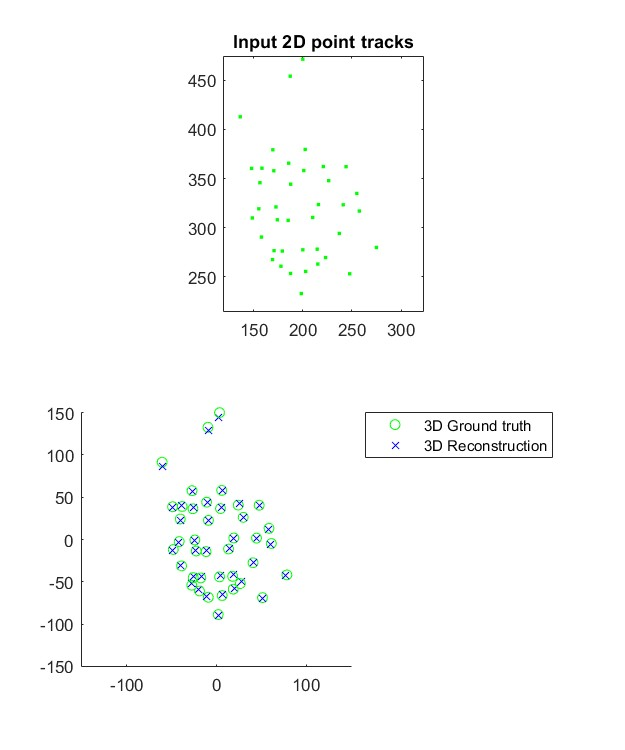
\includegraphics[width=\linewidth]{Figures/synthetic_reconstruction.jpg}
\caption{Synthetic 3D reconstruction}
\end{subfigure}
\hfill
\begin{subfigure}[b]{0.45\linewidth}
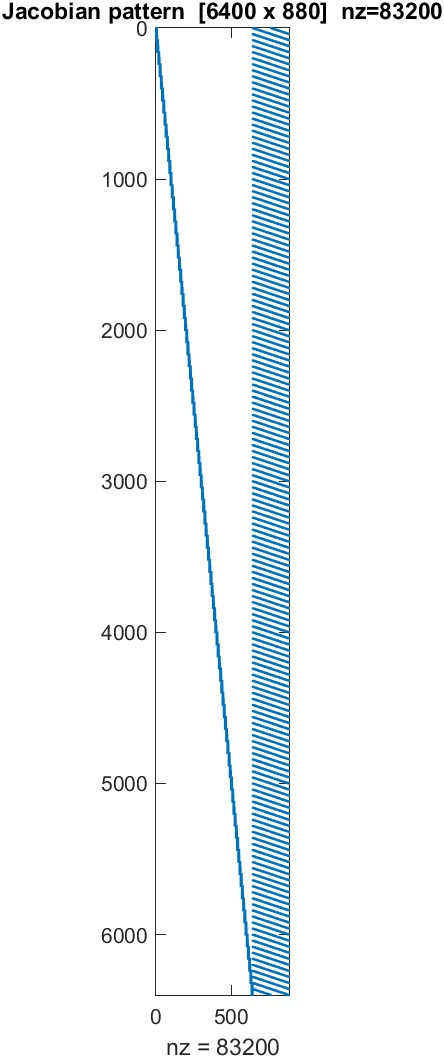
\includegraphics[width=\linewidth]{Figures/jacobian_synthetic.jpg}
\caption{Jacobian pattern (\texttt{spy(J)})}
\end{subfigure}
\caption{Results on the synthetic \texttt{face\_mocap.mat} sequence. Left: estimated 3D point cloud. Right: binary Jacobian pattern; each row corresponds to one residual and each column to one parameter; the block structure reflects the per-frame parameter grouping.}
\label{fig:synthetic_3Dreconstruction}
\end{figure}

\subsection{Non-Rigid Optimization: Real Sequence}

We then evaluate the same pipeline on the real \texttt{face\_real.mat} sequence, for which no 3D ground truth is available. Table~\ref{tab:real_errors} reports the 2D reprojection error before and after optimization.

\begin{table}[H]
\centering
\caption{2D reprojection errors on the real \texttt{face\_real.mat} sequence.}
\label{tab:real_errors}
\begin{tabular}{lc}
\toprule
 & 2D Reprojection Error \\
\midrule
Before optimization (rigid init.) & 0.56616\% \\
After optimization (non-rigid)    & 0.0030469\% \\
\bottomrule
\end{tabular}
\end{table}

The optimization again achieves a substantial reduction in reprojection error (from $0.566\%$ to $0.003\%$), consistent with the synthetic case. The higher initial error on the real sequence compared to the synthetic one reflects real-world noise and inaccuracies in the 2D tracking, which the non-rigid model must absorb.

\begin{figure}[H]
\centering
\begin{subfigure}[b]{0.45\linewidth}
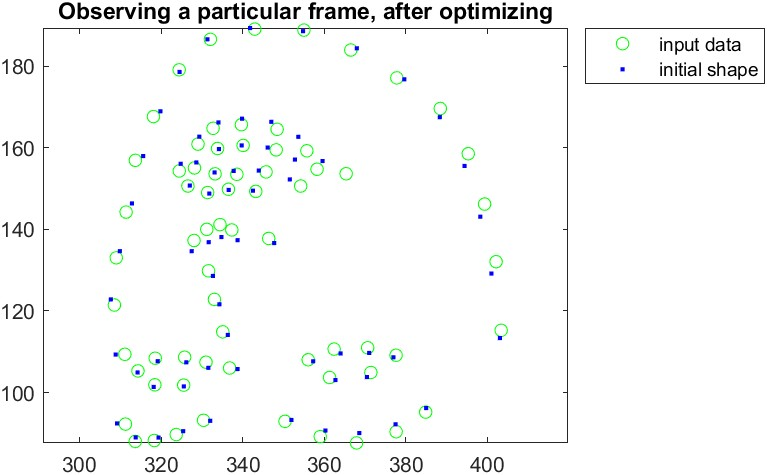
\includegraphics[width=\linewidth]{Figures/real_reconstruction.jpg}
\caption{Real 3D reconstruction}
\end{subfigure}
\hfill
\begin{subfigure}[b]{0.45\linewidth}
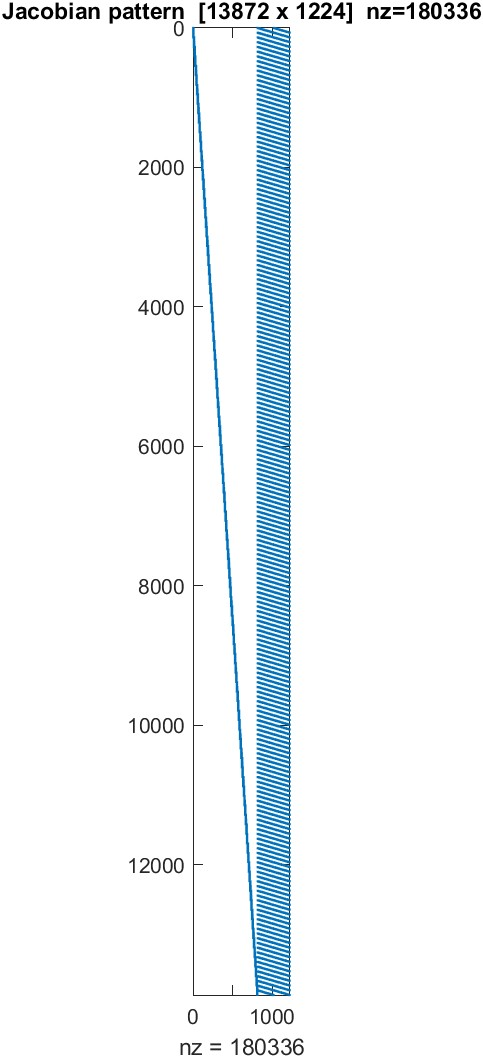
\includegraphics[width=\linewidth]{Figures/jacobian_real.jpg}
\caption{Jacobian pattern (\texttt{spy(J)})}
\end{subfigure}
\caption{Results on the real \texttt{face\_real.mat} sequence. Left: estimated 3D point cloud. Right: binary Jacobian pattern.}
\label{fig:real_3Dreconstruction}
\end{figure}

\subsection{Effect of Rank $K$ and Temporal Priors}

We study how the number of basis shapes $K$ and the temporal smoothness priors affect the Jacobian sparsity pattern on the synthetic \texttt{face\_mocap.mat} sequence.

\textbf{Effect of $K$.} As $K$ increases, each per-frame parameter block grows by one column (one additional coefficient $L_{k,f}$), and $K$ new rows of size $3P$ are appended to the basis section. Consequently the pattern becomes wider and the basis block in the lower-right corner grows, while the per-frame block structure in the upper-left remains similar in shape but with additional coefficient columns. Higher $K$ thus increases the number of non-zero entries in both the data rows (more coefficient dependencies) and the basis portion (more basis coordinate dependencies).

\textbf{Effect of temporal priors.} Activating the coefficient prior appends $F-1$ new rows at the bottom of the pattern, each connecting only the $K$ coefficient columns of two consecutive frames. Activating the camera prior similarly appends $F-1$ rows, each connecting only the 4 quaternion columns of two consecutive frames. In both cases the new rows are very sparse and form a distinctive banded structure beneath the main data block, as is clearly visible in the \texttt{spy} plots below.

\textbf{$K = 2$.}
\begin{figure}[H]
\centering
\begin{subfigure}[b]{0.45\linewidth}
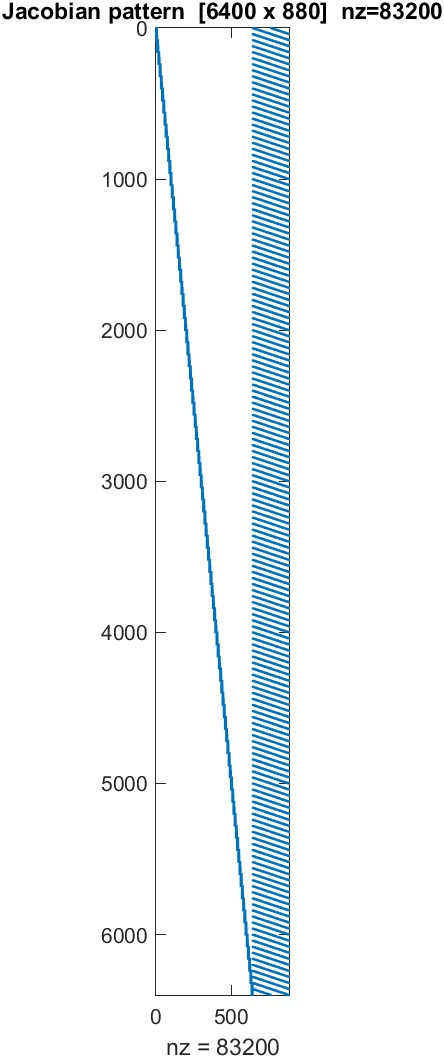
\includegraphics[width=\linewidth]{Figures/jacobian_K2_nopriors.jpg}
\caption{No priors}
\end{subfigure}
\hfill
\begin{subfigure}[b]{0.45\linewidth}
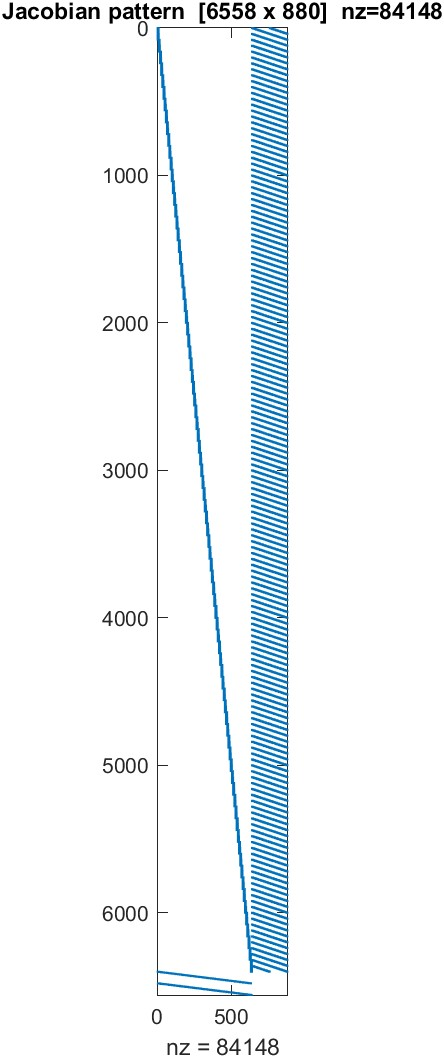
\includegraphics[width=\linewidth]{Figures/jacobian_K2_priors.jpg}
\caption{With both priors}
\end{subfigure}
\caption{Jacobian pattern for $K = 2$ with and without temporal priors. Activating the priors adds a sparse banded block at the bottom of the pattern.}
\label{fig:synthetic_reconstruction_K2}
\end{figure}

\textbf{$K = 3$.}
\begin{figure}[H]
\centering
\begin{subfigure}[b]{0.45\linewidth}
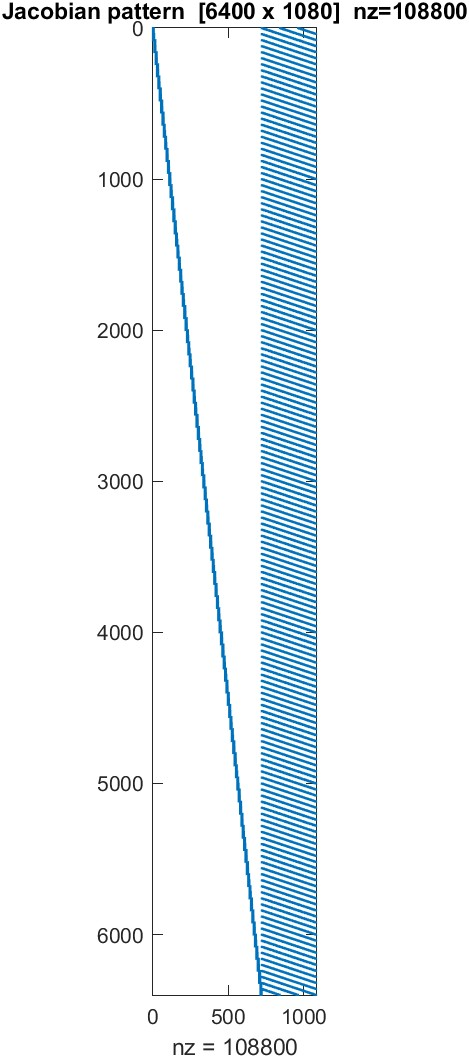
\includegraphics[width=\linewidth]{Figures/jacobian_K3_nopriors.jpg}
\caption{No priors}
\end{subfigure}
\hfill
\begin{subfigure}[b]{0.45\linewidth}
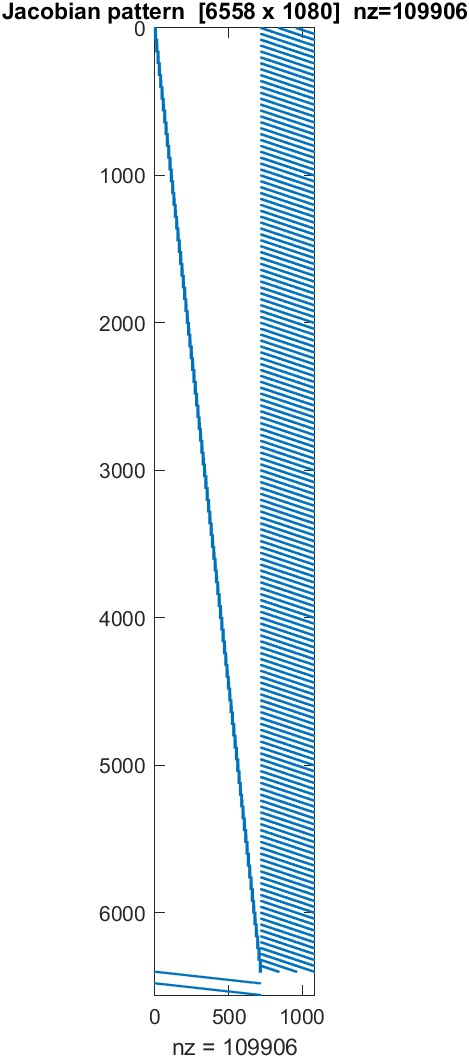
\includegraphics[width=\linewidth]{Figures/jacobian_K3_priors.jpg}
\caption{With both priors}
\end{subfigure}
\caption{Jacobian pattern for $K = 3$ with and without temporal priors. The per-frame block is wider than for $K=2$ due to the additional coefficient column.}
\label{fig:synthetic_reconstruction_K3}
\end{figure}

\textbf{$K = 4$.}
\begin{figure}[H]
\centering
\begin{subfigure}[b]{0.45\linewidth}
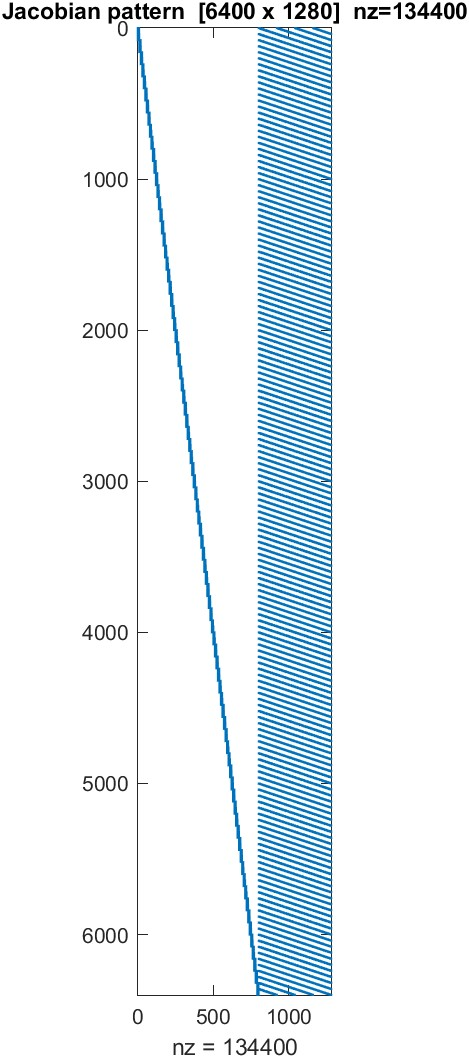
\includegraphics[width=\linewidth]{Figures/jacobian_K4_nopriors.jpg}
\caption{No priors}
\end{subfigure}
\hfill
\begin{subfigure}[b]{0.45\linewidth}
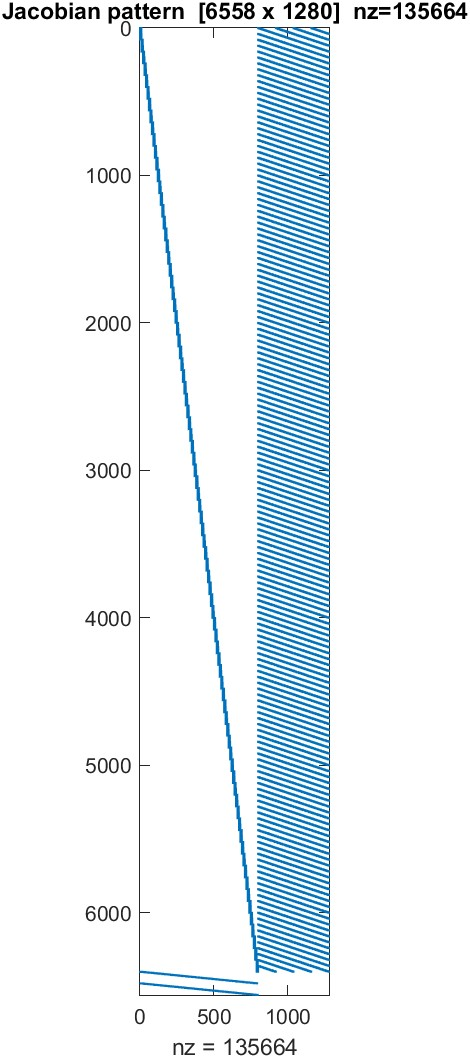
\includegraphics[width=\linewidth]{Figures/jacobian_K4_priors.jpg}
\caption{With both priors}
\end{subfigure}
\caption{Jacobian pattern for $K = 4$ with and without temporal priors. The basis block in the lower-right corner is now visibly larger, reflecting the four basis shapes and their $3P$ coordinates each.}
\label{fig:synthetic_reconstruction_K4}
\end{figure}

\subsection{Non-Rigid Structure from Motion by Trajectory Factorization}
Instead of modeling non-rigid shapes as linear combinations of basis profiles, the trajectory approach models the 3D path of each point over time using a predefined Discrete Cosine Transform (DCT) basis matrix $C \in \mathbb{R}^{F \times K}$. This models temporal smoothness directly within a lower-dimensional subspace.

Our completed implementation in \texttt{nrsfm\_trajectory.m} uses an initial SVD factorization truncated to a rank of $3K$, producing the uncalibrated factors $\hat{R}_{sh} \in \mathbb{R}^{2F \times 3K}$ and $\hat{X}_{hat} \in \mathbb{R}^{3K \times P}$. After using the metric upgrade step to determine matrix $Q$, the camera rotations $R$ are extracted via \texttt{recoverR.m}. The trajectory coefficients $D$ are then computed using a closed-form least-squares regression: $D = (G^T G)^{-1}G^T W$, where $G = R \cdot C$. Finally, the time-varying 3D shape is reconstructed via $X = C \cdot D$.

Table~\ref{tab:trajectory_metrics} shows the empirical data collected across all test sequences for model ranks $K \in \{2, \dots, 14\}$.

\begin{table}[H]
\centering
\caption{NRSfM Trajectory Factorization Performance Summary Across Sequences}
\label{tab:trajectory_metrics}
\begin{tabular}{lccc}
\toprule
\textbf{Sequence} & \textbf{Optimal Basis Rank ($K$)} & \textbf{Minimum 3D Error} & \textbf{Minimum Rotation Error} \\
\midrule
Drink    & 13 & 0.0249 & 0.0057 \\
Yoga     & 11 & 0.1624 & 0.1059 \\
Stretch  & 12 & 0.1087 & 0.0548 \\
Pickup   & 12 & 0.2368 & 0.1549 \\
Dance    & 5  & 0.2958 & N/A    \\
Dinosaur & 6  & 0.5997 & N/A    \\
\bottomrule
\end{tabular}
\end{table}

The optimal value of $K$ varies depending on the physical properties of each motion sequence. Sequences with highly repetitive or low-frequency paths (such as \textit{Dance} or \textit{Dinosaur}) compress effectively into lower-rank spaces ($K=5$ or $K=6$). In contrast, more complex or sudden movements (such as \textit{Drink} or \textit{Pickup}) require higher ranks ($K \ge 11$) to retain high-frequency components and minimize tracking residuals.

\subsection{Dinosaur Sequence Re-projection Visualization}
To validate the mathematical performance of our completed trajectory-space factorization pipeline under the identified optimal configuration ($K=6$), the derived solutions were fully integrated back into the verification script \texttt{visualize\_2Dtracking.m}. By isolating camera motion structures and temporal trajectories frame-by-frame, the recovered 3D point configurations were re-projected onto the 2D frame coordinate views via $W_{frame\_est} = R_{frame} \cdot S_{frame} + T_{frame}$. 

A representative sample of the synchronized tracking output from this optimization loop is provided in Figure~\ref{fig:dinosaur_trajectory_reprojection}. The continuous alignment of the model-derived paths against the empirical observation states indicates that the low-rank constraint stabilizes structural depth ambiguities while preventing catastrophic unobserved dimension collapse.

\begin{figure}[H]
\centering
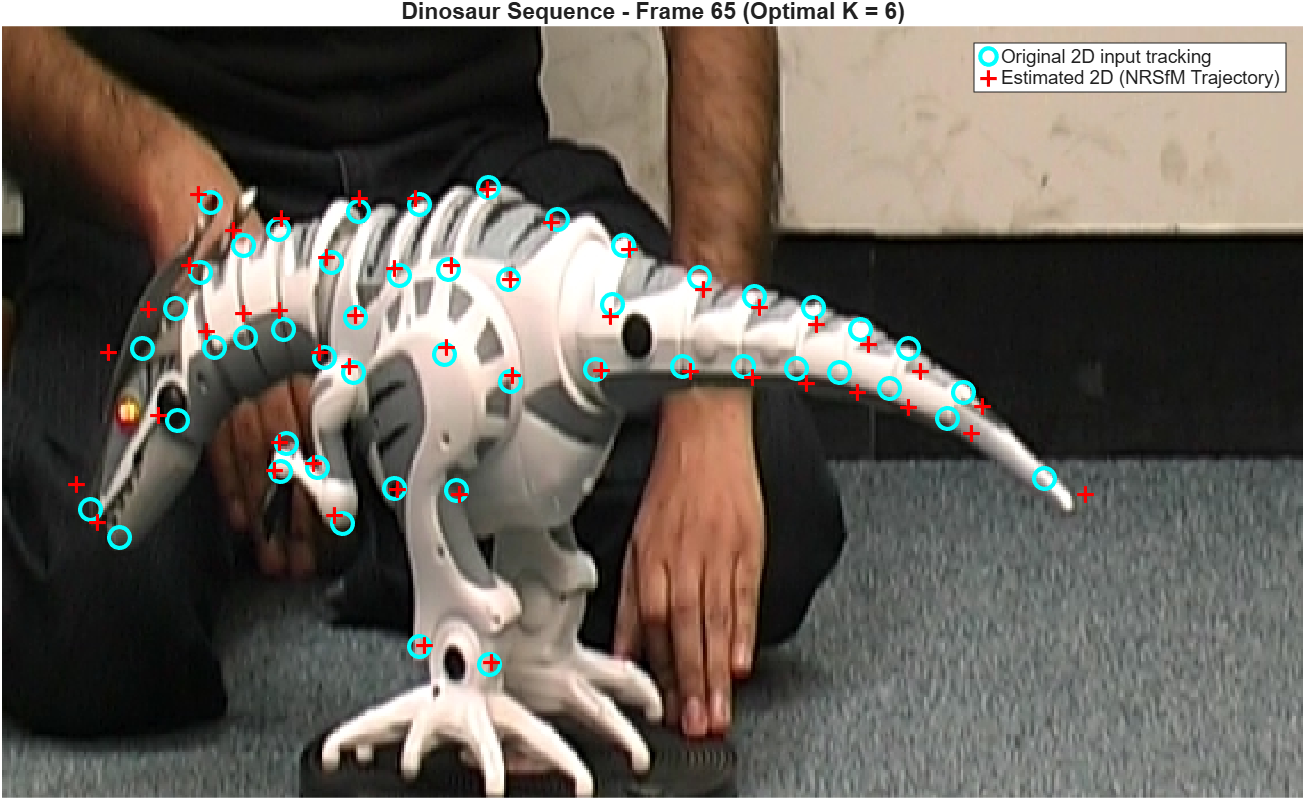
\includegraphics[width=0.65\linewidth]{Figures/dinosaur_estimated_overlay.png}
\caption{Visual comparison between original 2D feature tracking inputs (Cyan Circles) and the re-projected 2D trajectory estimation positions (Red Crosses) on the Dinosaur sequence ($K=6$).}
\label{fig:dinosaur_trajectory_reprojection}
\end{figure}


\section{Conclusion}
\label{sec:Conclusion}
This laboratory analyzed the progression from rigid camera factorization to deformable structure tracking. Rigid factorization remains highly precise for static objects, matching the Ogre sequence with a 3D reconstruction error of $0.002865\%$. For non-rigid shapes, unregularized optimization minimizing only 2D error leads to overfitting and distorts unobserved depth vectors. Incorporating spatial deformation constraints within the optimization Jacobian or projecting motion onto a low-rank temporal DCT trajectory basis suppresses these ambiguities. Finally, contemporary learning-based approaches replace explicit linear dimensions with continuous implicit manifolds, leveraging multi-objective constraints to reconstruct accurate 3D geometry from monocular video tracks.

\nocite{*}
\bibliographystyle{ieeetr}
\bibliography{references}

\end{document}